\section{Experimental Evaluation}

  In this section, we evaluate Lever's performance using various workloads. First, we describe the experimental environment, and then present the experimental results.

\subsection{Experimental Setup and Workloads}

  \textbf{Experimental Setup.} Our evaluations are conducted on a heterogeneous cluster consisting of two types of machines with different configurations. The first kind of machines is comprised of eight dual-core Intel Xeon E5-2670 2.6 GHZ CPUs(a total of 16 cores), 64GB memory, and 210GB disks. The second kind of machines consists of two dual-core 1.2 GHZ Intel CPU, 16GB memory, and 210GB disks. All computers are interconnected with 1Gbps Ethernet cards. We use spark-1.3.0 as the distributed computing platform and Redhat Enterprise Linux 6.2 with the kernel version 2.6.32 as the OS.

  \textbf{Workloads.} Table \uppercase\expandafter{\romannumeral2} describes the benchmarks used in our experiments. Similar to previous work \cite{Zaharia2013}, we choose three typical applications i.e. Grep, WordCount, and TopK. In addition, we also use the HiBench \cite{HiBench} benchmark including Identity, Sample and Projection. We rewrite the HiBench \cite{HiBench} benchmark based on receiver model.
  \begin{table*}[htbp]
    \footnotesize
    \centering
    \caption{Benchmarks}
    \begin{threeparttable}
    \centering
      \begin{tabular}{|p{1.4cm}|p{7.2cm}|p{1.5cm}|p{2.8cm}|p{1.7cm}|}
        \hline
        \centering
        \textbf{Benchmark} & \textbf{Description} & \textbf{Complexity} & \textbf{Resource Preference} & \textbf{Source} \\
        \hline
        Identity & Simply reads input and takes no operations on it & Single Step & None & HiBench \cite{HiBench} \\
        \hline
        Sample & Samples the input stream according to specified probability & Single Step & None & HiBench \cite{HiBench} \\
        \hline
        Projection & Extracts a certain field of the input & Single Step & Network Intensive & HiBench \cite{HiBench} \\
        \hline
        Grep & Checks if the input contains certain strings & Single Step & Network Intensive & DStream \cite{Zaharia2013} \\
        \hline
        WordCount & counts the number of each word in input text & Multi Step & CPU Intensive & DStream \cite{Zaharia2013} \\
        \hline
        Topk & Finds the k most frequent words over the specified window & Multi Step & CPU Intensive & DStream \cite{Zaharia2013} \\
        \hline
      \end{tabular}
    \end{threeparttable}
    \label{Table2}
  \end{table*}

  \textbf{Other configurations.} In all our experiments, we use default data locality wait time(3s), therefore Delay Scheduling \cite{Zaharia2010B} doesn't not interfere with our experimental results. For speculation, we set the speculation interval, speculation quantile(default 0.75) and speculation multiplier(default 1.5) as 100ms, 0.5, 1 respectively. These settings can let speculative execution perform much best in our environment. We implement Skewtune, Dolly and Wrangler's prototypes. We adopt local scan for skewtune. We also set wait duration of delay assignment $\omega$ as 200ms in Dolly. For Wrangler, we set confidence measure $\rho$ as 0.7 and set interval(decides how frequently a snapshot of node's resource usage counters is collected) $\Delta$ as one batch.

  Unless specified otherwise, we use 2s' batch interval and 100-bytes input records. Stragglers are on average 8 times slower than the median task in each job. All input data blocks only have one replica. We don't fetch the final results until the results are stable after each benchmark runs about 10 minutes. Each experiment is repeated five times and we present the median numbers. The baseline is original spark streaming with speculation closed.

\subsection{Job Completion Time}

  We first test the improvement in completion time using Lever. Figure 11 reports the normalized job completion time when compared with other strategies. Lever can significantly improve performance when running Projection, Grep, WordCount and Topk. But Lever improves a little for Identity and Sample relatively. It depends on the type of workloads. Identity and Sample are of simple execution logic. Straggler has little impact on these workloads.

  Compared to baseline, Lever improves the average job completion time by 32.31\%, 30.72\%, 37.54\% and 42.19\% for Projection, Grep, WordCount and Topk, respectively. Speculation and Skewtune works much worse in our experiments because they need to speed a long time on detecting stragglers and data skew. Lever pre-schedules job input data before task scheduling and avoid the detecting and migrating overhead. As a result, Lever outperforms other strategies for the performance of Projection(by up to 29.47\%, 32.06\%, 22.99\% and 25.56\% compared to Speculation, Skewtune, Dolly and Wrangler), Grep(by up to 28.87\%, 29.11\%, 18.82\% and 25.81\% compared to Speculation, Skewtune, Dolly and Wrangler), WordCount(by up to 33.33\%, 37.37\%, 31.11\% and 28.74\% compared to Speculation, Skewtune, Dolly and Wrangler) and Topk(by up to 34.48\%, 41.24\%, 34.48\% and 31.33\% compared to Speculation, Skewtune, Dolly and Wrangler).
  \begin{figure}[htbp]
    \centering
    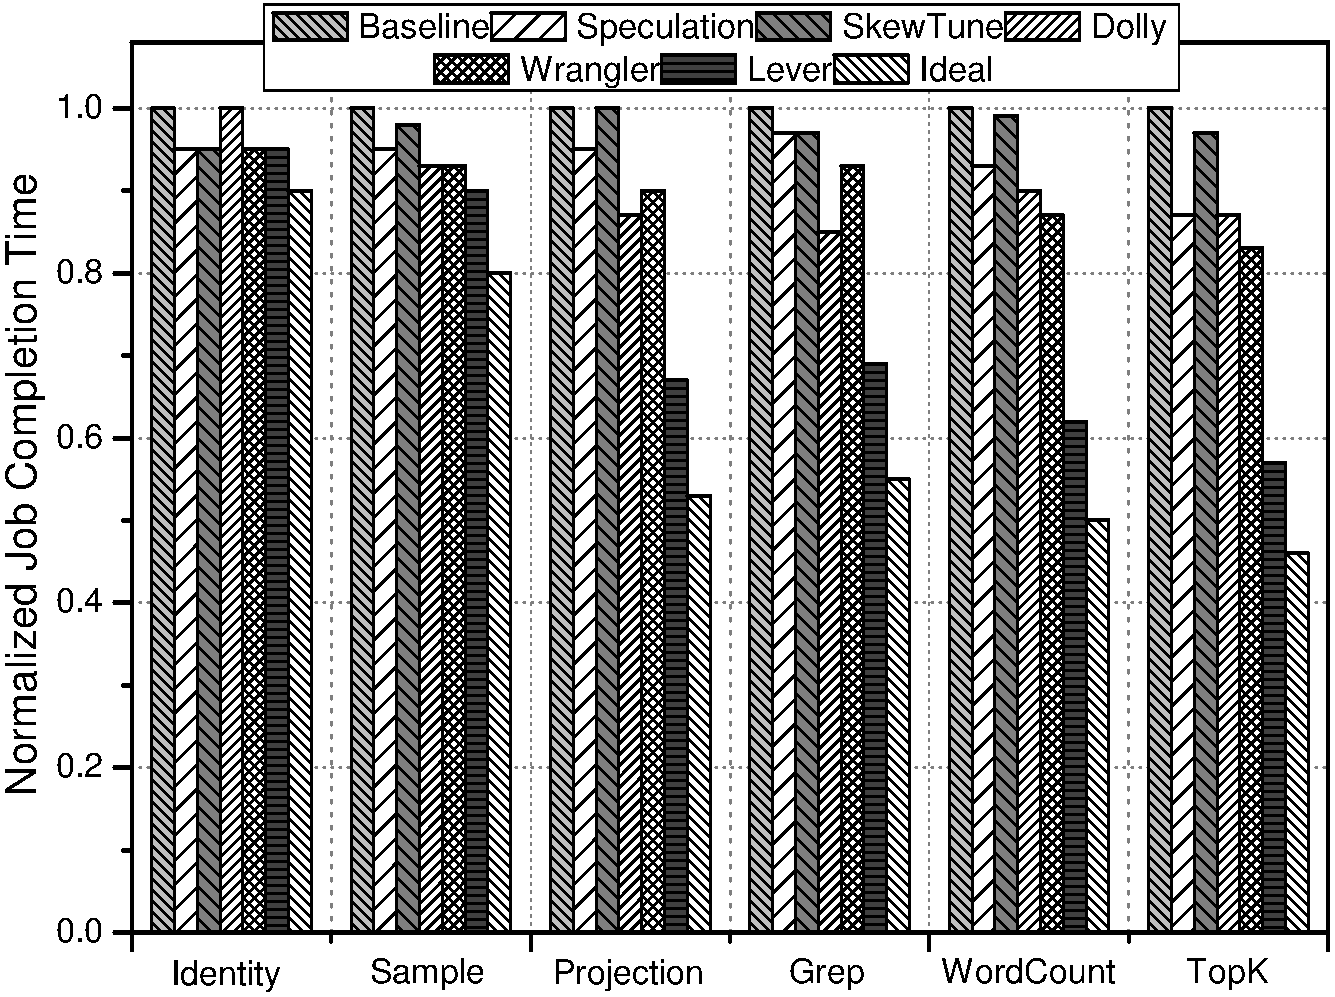
\includegraphics[width=0.35\textwidth]{FigureJCT}
    \caption{Normalized job completion time when running benchmarks under different techniques}
    \label{Fig. 11:}
  \end{figure}

  Figure 12 shows a detailed analysis of task completion time in three types of nodes. We average task's completion time of faster group, median group and straggler group. Task's completion time in each node decides the makespan of this job. As we can see, straggler is quite remarkable under traditional methods. It means that these techniques cannot eliminate stragglers very well. As a result, the straggler nodes are load-heavy all the batch and the fasters are idle for a long time. It is due to their fumbling reaction to stragglers. In the ideal case, all the nodes should complete their tasks at almost the same time. Lever behaviors much better because it balances data skew when receiving data. So when tasks are running, all nodes can progress at almost the same rate.
  \begin{figure}[htbp]
    \centering
    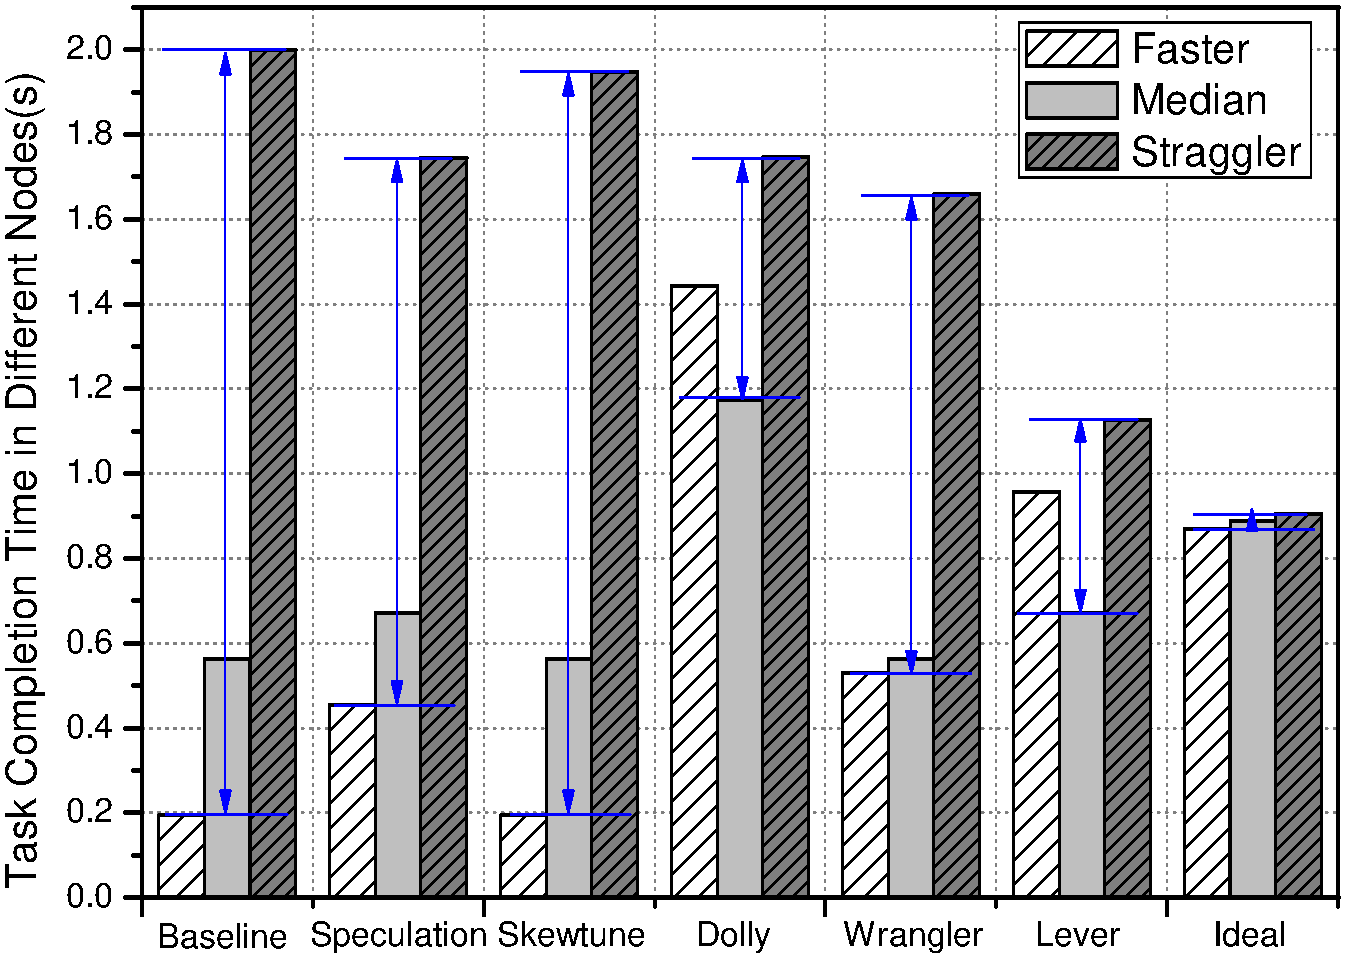
\includegraphics[width=0.32\textwidth]{FigureMakeSpan}
    \caption{Task completion time in three types of nodes when running WordCount}
    \label{Fig. 12:}
  \end{figure}

  Table \uppercase\expandafter{\romannumeral3} lists the node's idle time when a batch is completed. Baseline and Skewtune waste more than 3s for faster and median nodes totally in a 2s' batch interval. Speculation and Wrangler are idle for about 2s. Much of this time is spent on detection and migration. This is the root cause of why they perform much worse than others. Although Dolly wastes less time, it clones tasks, which means that it need to complete 2x amount of work. Lever also has idle time as long as 0.625s. This is because Lever only takes the straggler and faster into account regardless of median group's node. For median, it is difficult to estimate whether it will be faster or slower than stragglers after we redistribute load.
  \begin{table*}[htbp]
    \small
    \centering
    \caption{Node's idle time for faster and median}
    \begin{threeparttable}
    \centering
      \begin{tabular}{|p{1.4cm}|p{1.2cm}|p{1.5cm}|p{1.2cm}|p{0.9cm}|p{1.2cm}|p{0.9cm}|p{0.9cm}|}
        \hline
        Techniques & Baseline & Speculation & Skewtune & Dolly & Wrangler & Lever & Ideal \\
        \hline
        Idle time & 3.243s & 2.363s & 3.137s & 0.875s & 2.224s & 0.625s & 0.055s \\
        \hline
      \end{tabular}
    \end{threeparttable}
    \label{Table3}
  \end{table*}

  In summary, Lever saves a lot of idle time through pre-scheduling data assignment, thus avoiding detection, migration and cloning. So Lever can mitigate stragglers and improve the performance significantly.

\subsection{Adaptability for burst load}

  In this testing scenario, we give one node burst load to evaluate the robustness and the convergence time of Lever. The burst load results in that task completion time exceeds greatly than batch interval. We also test other techniques' effectiveness under this situation.

  From the test result in Figure 13, we observe that both Lever and Wrangler can achieve much better performance. Baseline, Speculation, Skewtune and Dolly can't process subsequent jobs timely because their cloning and hysteresis reaction aren't not enough, leading a large number of subsequent jobs are queueing in scheduler's waiting queue. The scheduling delay will increases monotonously.

  Although Wrangler can go on processing subsequent jobs, Wrangler is not stable enough with delay jitter. This is because Wrangler only cares about stragglers in one batch. The nodes of light load(actually are potential stragglers) in current batch will be scheduled many tasks in the next batch, leading to nodes being overloaded.

  Lever avoids this problem by analyzing recurring jobs' load fluctuation in previous batches. As shown in Figure 13, Lever can converge to an ideal latency in six batches. The estimation for capability by using ILC also returns to normal in six batches after experiencing a short period of fluctuations.

  In summary, Lever can adapt to burst load effectively and converge to a steady state quickly.
  \begin{figure}[htbp]
    \centering
    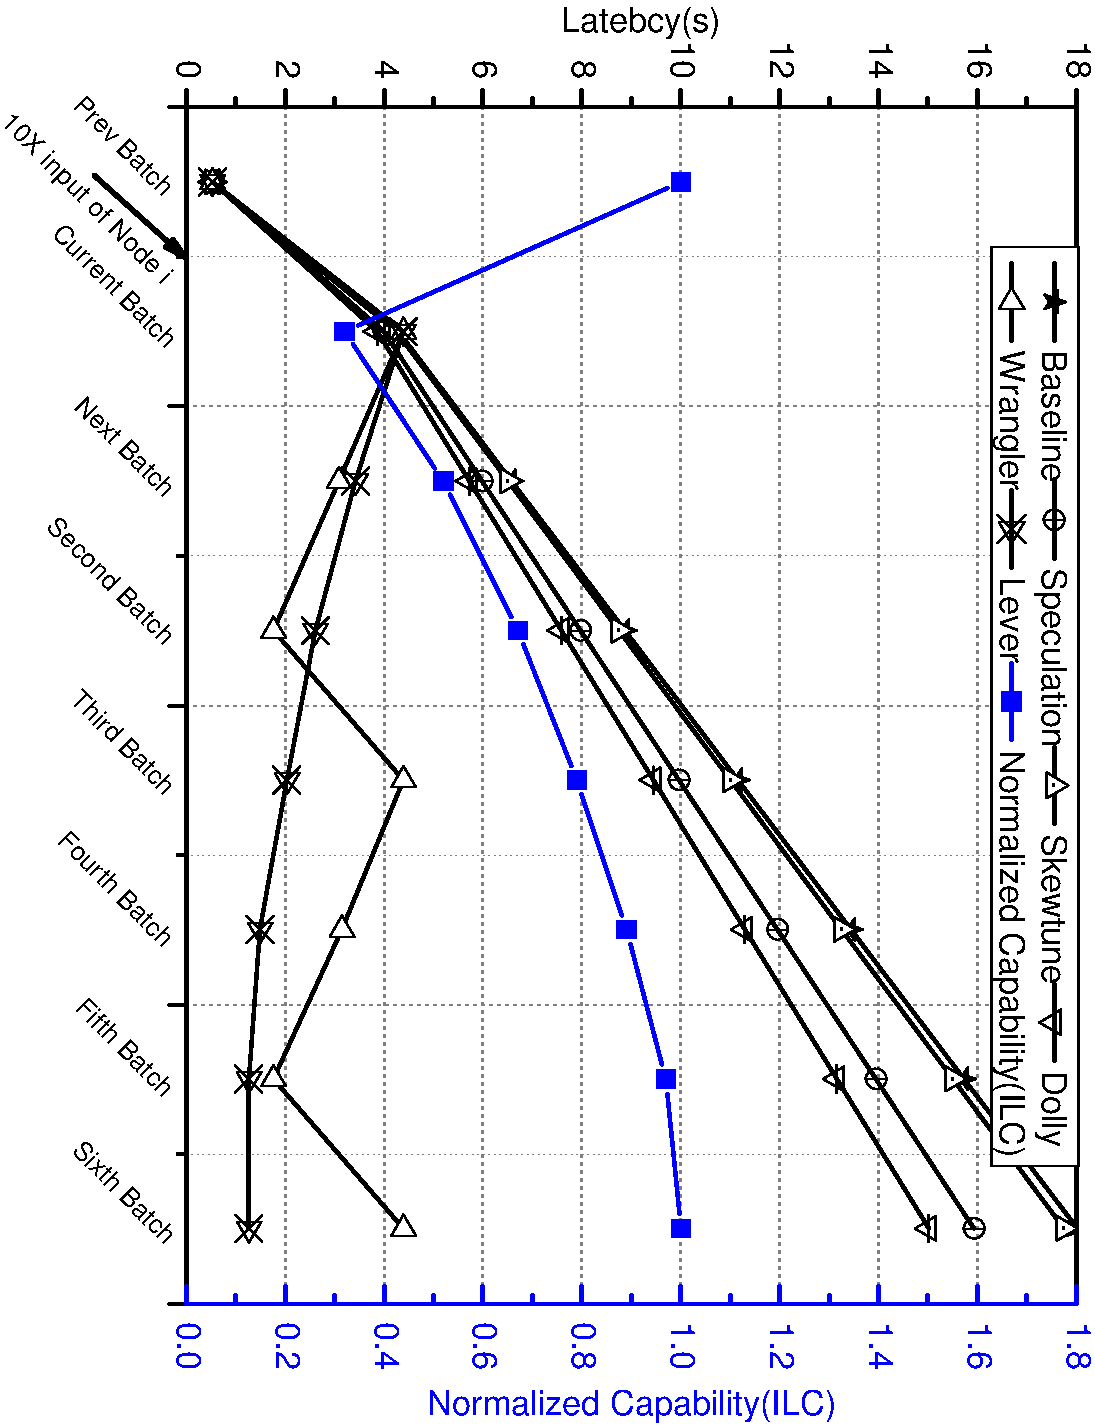
\includegraphics[width=0.30\textwidth, angle=90]{FigureAdapBurst}
    \caption{Latency and Normalized Capability when running WordCount under burst load}
    \label{Fig. 13:}
  \end{figure}

\subsection{Data Locality and Queued Tasks}

  \begin{figure}[htbp]
    \centering
    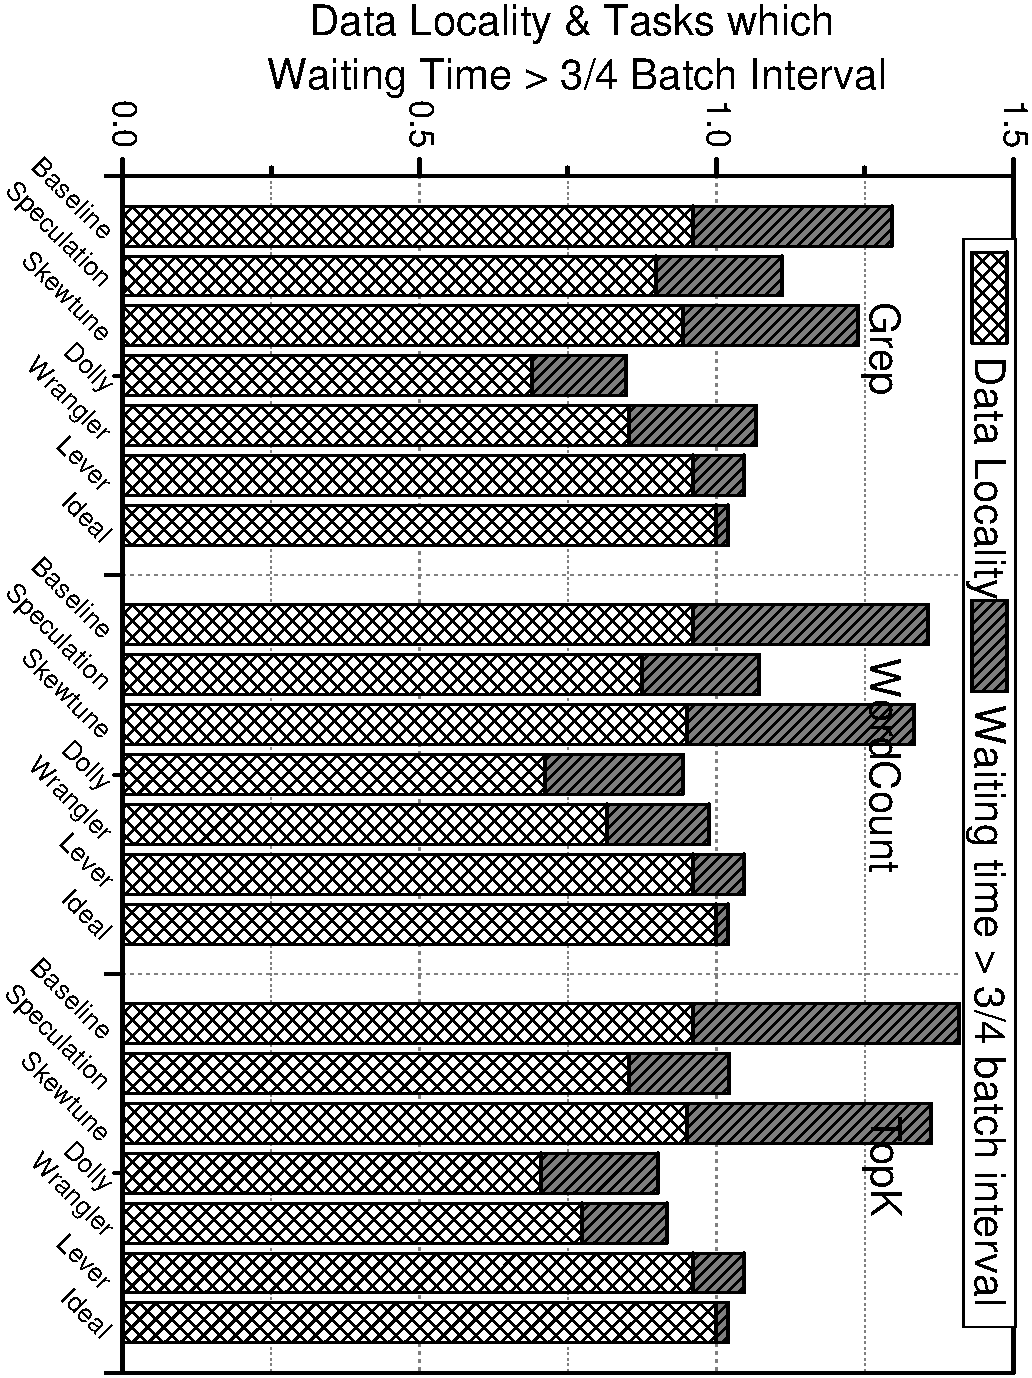
\includegraphics[width=0.28\textwidth, angle=90]{FigureDLWT}
    \caption{Data Locality and Tasks which waiting time is greater than 3/4 batch interval when running Grep, WordCount and Topk}
    \label{Fig. 14:}
  \end{figure}

  In this test, we conduct a statistical analysis about data locality and queued tasks which waiting time is greater than three quarters of batch interval. We observe that in our experiments if a task waits for three quarters of batch interval, it means that this node is overloaded and the batch processing time will exceed the batch interval.

  As shown in Figure 14, for Baseline, although most of the tasks can execute in the local node, there are 33.5\%, 39.7\%, 44.9\% tasks waiting for more than three quarters of batch interval for Grep, WordCount and Topk, respectively. These tasks are from straggler nodes. In order to illustrate the difference, we take WordCount for example. Dolly and Wrangler only have up to 23.1\% and 17.3\% tasks waiting for more than three quarters of batch interval. However, they only have 71.2\% and 81.5\% node local tasks. They need to migrate tasks to remote nodes at runtime. This migration causes extra overhead and neutralizes benefits from reduction in the number of waiting tasks. Speculation only detects and migrates a small number of tasks. Skewtune performs much worse because it spends so long time on detection that it can't react to straggler and data skew quickly.

  In the ideal case, all nodes execute local tasks and there aren't tasks queued for three quarters of batch interval. Lever can achieve 96\% data locality and 8.7\% waiting tasks. The reason why Lever can not reach the ideal state is that Lever relies on the estimation of node's capability and Lever ignores the median nodes. This impedes Lever's perfect load balancing.

  In summary, compared to other strategies, Lever can achieve better data locality and reduce the number of tasks which waiting for a long time.

\subsection{All Strategy or Two Choice Strategy}

  In this test scenario, we compare two helper-choosing strategies when faced with different straggler situations. We varies the number of stragglers and the number of fasters to evaluate the advantages and disadvantages of two methods.

  The experimental results presented in Figure 15 show that when there are few stragglers in current cluster, allStrategy is much better than twoChoiceStrategy. However, if there are more and more nodes will be stragglers, twoChoiceStrategy behave much better. We give an example to elaborate the reason. Assume that we have n stragglers and m fasters, allStrategy produces n$\times$m partitions to migrated and rebalanced, but twoChoiceStrategy only produces n$\times$2 fragmentations. Although allStrategy makes load well-distributed, which accompany with it is the increasing overhead in partition and network transformation.

  In our experiments, when there are 8 stragglers and 10 fasters, twoChoiceStrategy begins to perform better than allStrategy. It means that when the observed value $\rho$ is larger than 80, then Lever should choose twoChoiceStrategy. As shown in Figure 15, Lever can select helper-choosing strategies adaptively according to straggler situations and latency fluctuation.
  \begin{figure}[htbp]
    \centering
    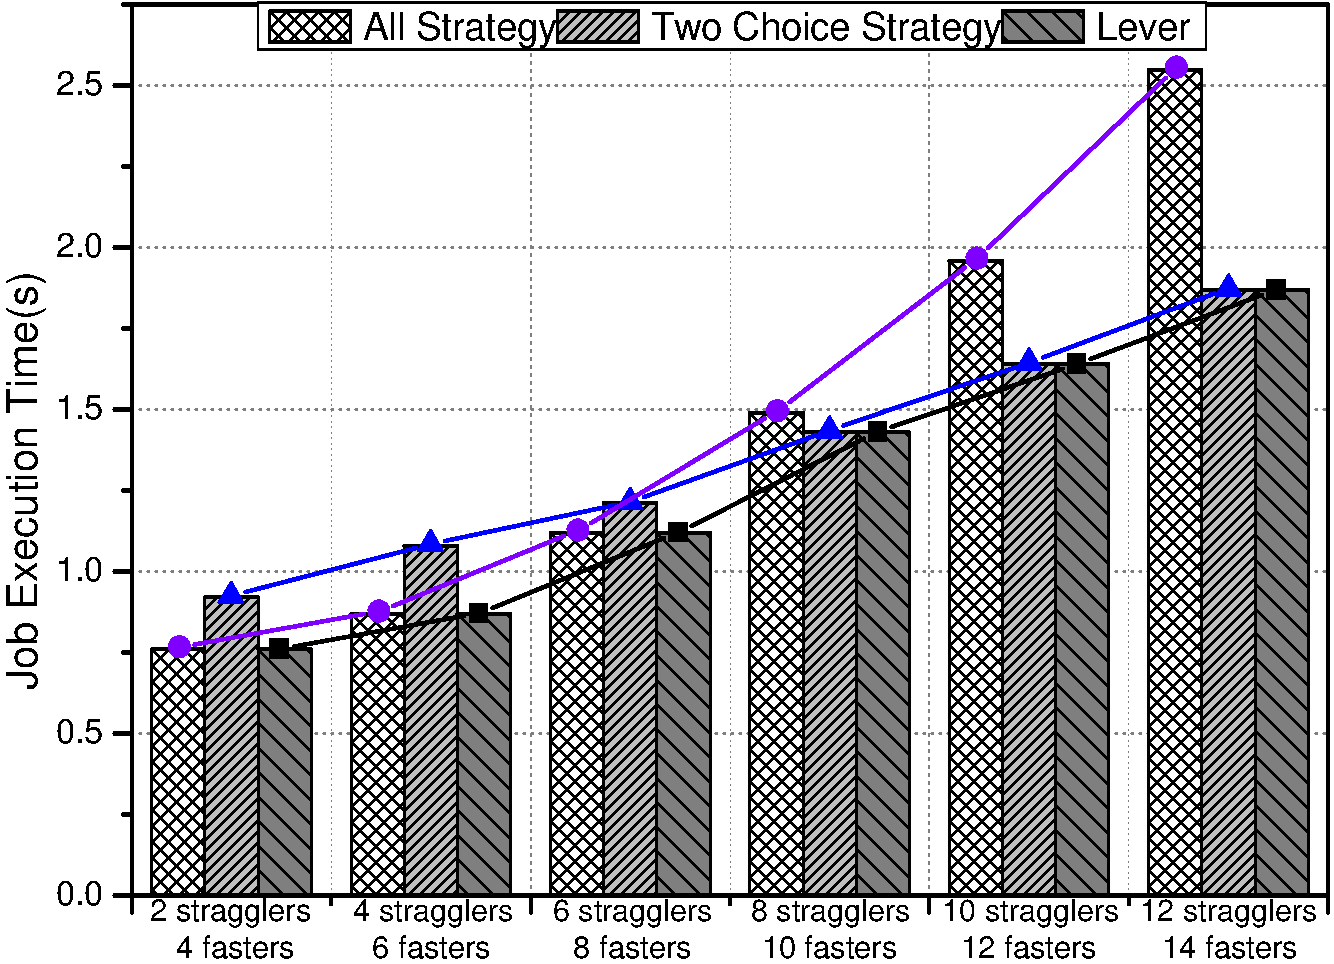
\includegraphics[width=0.35\textwidth]{FigureAllorTwo}
    \caption{Results under different straggler situations using two strategies}
    \label{Fig. 15:}
  \end{figure}

  In summary, allStrategy is suitable for few stragglers and few fasters and twoChoiceStrategy is more suitable for many stragglers or many fasters. Lever can choose one of the two adaptively to ensure the performance.